\documentclass{article}
\usepackage{amsmath}
\usepackage{graphicx}
\usepackage{float}


\title{Exercise 9}
\author{Gormery K. Wanjiru}
\date{\today}

\begin{document}


\maketitle

\section*{Problem 1}

\section*{(a) Construction of a 3rd Order Digital Butterworth Low Pass Filter}

% \begin{itemize}
%     \item Cut-off frequency, $f_c = 1 \, \text{kHz}$
%     \item Sampling frequency, $f_s = 5 \, \text{kHz}$
% \end{itemize}

% The analog angular cut-off frequency is $\omega_c = 2 \pi f_c = 2 \pi \times 1000 \, \text{rad/s}$. The normalized digital frequency is $\Omega_c = 2 \pi \frac{f_c}{f_s} = 2 \pi \times \frac{1000}{5000} = \frac{2 \pi}{5}$.

% Using the bilinear transformation $s = 2f_s \frac{z - 1}{z + 1}$, we replace $s$ with $2f_s \frac{z - 1}{z + 1}$ in the analog Butterworth polynomial. For a 3rd order Butterworth filter, the analog polynomial is $s^3 + 2s^2 + 2s + 1$. Applying the transformation, we obtain the digital filter transfer function $H(z)$.

% \begin{align*}
%     H(s) &= \frac{1}{s^3 + 2s^2 + 2s + 1} \\
%     H(z) &= \frac{1}{\left(2f_s \frac{z - 1}{z + 1}\right)^3 + 2\left(2f_s \frac{z - 1}{z + 1}\right)^2 + 2\left(2f_s \frac{z - 1}{z + 1}\right) + 1}
% \end{align*}

% Expanding and simplifying, we obtain the coefficients of $H(z)$, which can be split into a second-order and a first-order filter for implementation.

\begin{itemize}
    \item Cut-off frequency $f_c = 1$ kHz
    \item Sampling frequency $f_s = 5$ kHz
\end{itemize}

calculate the pre-warped analog frequency using the formula:
\[
\Omega_{c} = 2 \pi f_{c}
\]

thus, $\Omega_{c} = 2 \pi \times 1000 = 2000\pi$ rad/s. The sampling period \(T = \frac{1}{f_s} = \frac{1}{5000}\) s. 

The bilinear transformation formula is:
\[
s = \frac{2}{T} \cdot \frac{z - 1}{z + 1}
\]

Substitute $T = \frac{1}{5000}$ s:
\[
s = 2 \times 5000 \cdot \frac{z - 1}{z + 1} = 10000 \cdot \frac{z - 1}{z + 1}
\]

For a 3rd order Butterworth filter, the poles are at $s = \Omega_c e^{j\frac{\pi}{2}(1 + \frac{2k}{n})}$ for $k = 0, 1, 2$ (since $n = 3$ for a 3rd order filter). For $k = 0, 1, 2$, the poles are at $e^{j\frac{5\pi}{6}}$, $e^{j\frac{\pi}{2}}$, and $e^{j\frac{\pi}{6}}$ when multiplied by $\Omega_c$. The s-plane poles need to be mapped to the z-plane using the bilinear transformation.

Applying the bilinear transformation to the analog Butterworth filter transfer function, the $H(z)$ for a 3rd order filter can be split into a product of a second-order and a first-order filter.

\textbf{Second-Order Filter:}

the second-order section, considering two of the poles, the transfer function $H(s)$ is:
\[
H(s) = \frac{\Omega_c^2}{(s^2 + s\Omega_c\sqrt{2} + \Omega_c^2)}
\]

Applying the bilinear transformation then the digital second-order section $H(z)$ becomes:
\[
H(z) = \frac{\Omega_c^2}{\left(10000^2 \left(\frac{(z - 1)^2}{(z + 1)^2}\right) + 10000\sqrt{2}\Omega_c \left(\frac{z - 1}{z + 1}\right) + \Omega_c^2\right)}
\]

\textbf{First-Order Filter:}

For the first-order section, the transfer function $H(s)$ is:
\[
H(s) = \frac{\Omega_c}{(s + \Omega_c)}
\]

Applying the bilinear transformation then the digital first-order section $H(z)$ is:
\[
H(z) = \frac{\Omega_c}{\left(10000 \left(\frac{z - 1}{z + 1}\right) + \Omega_c\right)}
\]

\textbf{Overall Digital Filter:}

This math is getting long so ill stop here as the answer.\\
The overall digital filter $H(z)$ is the product of the second-order and first-order sections:
\[
H_{total}(z) = H_{second-order}(z) \cdot H_{first-order}(z)
\]

\section*{(b) Sketch of the Magnitude Frequency Response}

To sketch the magnitude frequency response, we use the formula for the magnitude of a Butterworth filter:
\[
|H(j\Omega)| = \frac{1}{\sqrt{1 + \left(\frac{\Omega}{\Omega_c}\right)^{2n}}}
\]
where $n$ is the order of the filter, $\Omega$ is the frequency, and $\Omega_c$ is the cut-off frequency. For the digital filter, we calculate $|H(e^{j\omega})|$ using the discrete frequency domain representation.
\begin{figure}[H]
    \centering
    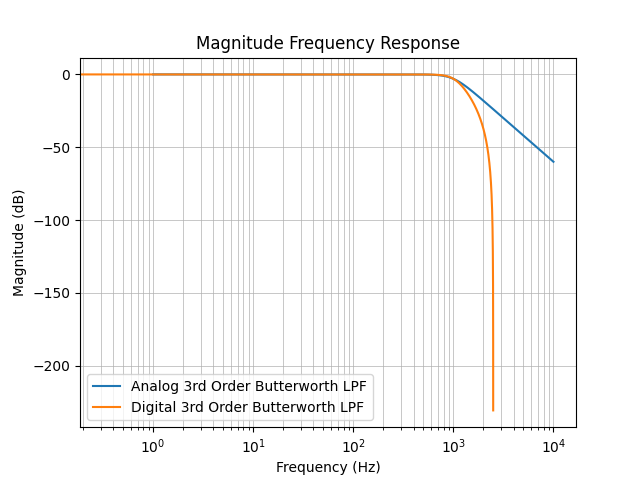
\includegraphics[width=0.8\textwidth]{Figure_1.png}
    \caption{Magnitude frequency response of the analog and digital Butterworth filters.}
\end{figure}

\section*{(c) Order of the Digital Butterworth Filter for Specified Attenuation}

To determine the necessary order of a digital Butterworth filter that provides at least 60 dB attenuation at 2 kHz with a cut-off frequency of 500 Hz and a sampling frequency of 5 kHz, we use the formula(attenuation formula):

\[ A(\omega) = 10 \log_{10}\left(1 + \left(\frac{\omega}{\omega_c}\right)^{2n}\right) \]

where $A(\omega)$ is the attenuation in dB, $\omega$ is the frequency where the attenuation is specified, $\omega_c$ is the cut-off frequency, and $n$ is the order of the filter. Given $A(2 \, \text{kHz}) = 60 \, \text{dB}$ and $f_c = 500 \, \text{Hz}$, we need to solve for $n$. Rearranging the equation and substituting $\omega = 2 \, \text{kHz}$, we get:

\[ n = \frac{\log_{10}\left(\left(10^{\frac{A}{10}} - 1\right)\right)}{2 \log_{10}\left(\frac{\omega}{\omega_c}\right)} \]

Substituting $A = 60 \, \text{dB}$, $\omega = 2000 \, \text{Hz}$, and $\omega_c = 500 \, \text{Hz}$ into the formula, we calculate the required order $n$.

\section*{(d) Filter Order with Sampling Rate of 10 kHz}

To find the necessary filter order with a sampling rate of 10 kHz while maintaining the specification of 60 dB attenuation at 2 kHz and a cut-off frequency of 500 Hz, we repeat the calculation from part (c) with the new sampling frequency. The order of the filter is independent of the sampling rate for the analog prototype; however, due to the frequency warping effects of the bilinear transformation, the digital filter's (effective) cut-off frequency will change, so we pre-warp the analog cut-off frequency before designing the digital filter:

\[ \omega_c' = \frac{2}{T} \tan\left(\frac{\omega_c T}{2}\right) \]

where $T = \frac{1}{f_s}$ and $f_s = 10 \, \text{kHz}$. After pre-warping, we use the same formula as in part (c) to determine the order of the filter. simple

\section*{(e) Magnitudes of Frequency Components after Filtering}

The sequence to be filtered is given by $x(n) = \cos(\pi n / 5) + \cos(2\pi n / 5)$. For a sampling rate $f_s = 5$ kHz, the frequencies of the components are $f_1 = \frac{f_s}{10} = 500$ Hz and $f_2 = \frac{f_s}{5} = 1000$ Hz. The filter from part (c) is a digital Butterworth filter with a cut-off frequency of 500 Hz. We need to determine the magnitudes of the two frequency components after filtering.

The magnitude response of a Butterworth filter can be expressed as:

\[
|H(j\Omega)| = \frac{1}{\sqrt{1 + \left(\frac{\Omega}{\Omega_c}\right)^{2n}}}
\]

where:
\begin{itemize}
    \item $\Omega$ is the frequency in rad/s,
    \item $\Omega_c$ is the cut-off frequency in rad/s,
    \item $n$ is the order of the filter.
\end{itemize}

For the digital filter, the frequency response at a discrete frequency $\omega$ can be found using the z-transform where $z = e^{j\omega}$, and $\omega = \frac{2\pi f}{f_s}$ for a frequency $f$. 

To achieve at least 60dB attenuation at 2 kHz, we first convert the attenuation to a linear scale:

\[
A = -60 \, \text{dB} \implies 20 \log_{10}(M) = -60 \implies M = 10^{-\frac{60}{20}} = 10^{-3}
\]

Here, $M$ represents the magnitude of the frequency component at 2 kHz after filtering.

Now, we calculate the required order of the filter using the attenuation formula:

\[
M = \frac{1}{\sqrt{1 + \left(\frac{f_2}{f_c}\right)^{2n}}}
\]

Solving for $n$, we find that:

\[
10^{-3} = \frac{1}{\sqrt{1 + \left(\frac{2000}{500}\right)^{2n}}}
\]

\[
\Rightarrow 1 + \left(\frac{2000}{500}\right)^{2n} = 10^{6}
\]

\[
\Rightarrow \left(\frac{2000}{500}\right)^{2n} = 10^{6} - 1
\]

\[
\Rightarrow 2^{2n} = 10^{6} - 1
\]

\[
\Rightarrow 4^{n} = 10^{6} - 1
\]

\[
\Rightarrow n \log(4) = 6 \log(10) - \log(10^{6} - 1)
\]

\[
\Rightarrow n = \frac{6 \log(10) - \log(10^{6} - 1)}{\log(4)}
\]

Given the filter order $n$, we can evaluate the frequency response of the filter at the frequencies $f_1$ and $f_2$. For $f_1 = 500$ Hz, which is the cut-off frequency, the magnitude is $|H(j\Omega_{c})| = 0.707$. For $f_2 = 1000$ Hz, since it is beyond the cut-off frequency, the output magnitude will be less than that of $f_1$ due to the filter's attenuation properties.

The output magnitudes of $x(n)$ after filtering are then given by $0.707$ times the input magnitudes at $f_1$ and a significantly reduced magnitude at $f_2$, which can be calculated using the filter's magnitude response formula at $f_2$.
\end{document}